\documentclass{article}

% if you need to pass options to natbib, use, e.g.:
\PassOptionsToPackage{numbers, compress, sort}{natbib}
% before loading neurips_2021

% ready for submission
%\usepackage{neurips_2021}

% to compile a preprint version, e.g., for submission to arXiv, add the
% [preprint] option:
%\usepackage[preprint]{neurips_2021}
\usepackage{neurips_2021}

% to compile a camera-ready version, add the [final] option, e.g.:
%     \usepackage[final]{neurips_2021}

% to avoid loading the natbib package, add option nonatbib:
%    \usepackage[nonatbib]{neurips_2021}

\usepackage[utf8]{inputenc} % allow utf-8 input
\usepackage[T1]{fontenc}    % use 8-bit T1 fonts
\usepackage{hyperref}       % hyperlinks
\usepackage{url}            % simple URL typesetting
\usepackage{booktabs}       % professional-quality tables
\usepackage{amsfonts}       % blackboard math symbols
\usepackage{nicefrac}       % compact symbols for 1/2, etc.
\usepackage{microtype}      % microtypography
\usepackage{xcolor}         % colors
\usepackage{enumitem}

\title{Fat--Tailed Variational Inference with \\ Anisotropic Tail Adaptive Flows}

% The \author macro works with any number of authors. There are two commands
% used to separate the names and addresses of multiple authors: \And and \AND.
%
% Using \And between authors leaves it to LaTeX to determine where to break the
% lines. Using \AND forces a line break at that point. So, if LaTeX puts 3 of 4
% authors names on the first line, and the last on the second line, try using
% \AND instead of \And before the third author name.

\author{%
  Feynman Liang\\
  Department of Statistics\\
  University of California, Berkeley\\
  \texttt{feynman@berkeley.edu} \\
  \And
  Liam Hodgkinson\\
  ICSI and Department of Statistics\\
  University of California, Berkeley\\
  \texttt{liam.hodgkinson@berkeley.edu} \\
  \And
  Michael W. Mahoney\\
  ICSI and Department of Statistics\\
  University of California, Berkeley\\
  \texttt{mmahoney@stat.berkeley.edu} \\
}


\usepackage{amssymb,amsmath,amsthm}
\newtheorem{theorem}{Theorem}
\theoremstyle{definition}
\newtheorem{definition}[theorem]{Definition}
\newtheorem{assumption}[theorem]{Assumption}
\newtheorem{proposition}[theorem]{Proposition}
\newtheorem{lemma}[theorem]{Lemma}
\newtheorem{claim}[theorem]{Claim}
\newtheorem{example}[theorem]{Example}
\newtheorem{corollary}[theorem]{Corollary}

\theoremstyle{remark}
\newtheorem{remark}[theorem]{Remark}


\usepackage[bold]{hhtensor}


% \usepackage{natbib}
\bibliographystyle{abbrv}
% \usepackage{hyperref}
\usepackage{cleveref}
\usepackage{mathtools}
\usepackage{booktabs}
\usepackage{float}
\usepackage{braket}
\usepackage{dsfont}
\usepackage{graphbox}
\usepackage{pgf}
\usepackage{comment}
\usepackage{subcaption}

\crefname{assumption}{assumption}{assumptions}
\Crefname{assumption}{Assumption}{Assumptions}
\crefname{proposition}{proposition}{propositions}
\Crefname{proposition}{Proposition}{Propositions}
\crefname{lemma}{lemma}{lemmas}
\Crefname{lemma}{Lemma}{Lemmas}
\crefname{remark}{remark}{remarks}
\Crefname{remark}{Remark}{Remarks}

\DeclarePairedDelimiterX{\infdivx}[2]{(}{)}{%
  #1\;\delimsize\|\;#2%
}
\newcommand{\infdiv}{D\infdivx}

\DeclareMathOperator*{\cov}{cov}

\newcommand{\dd}{\mathrm{d}}

\newcommand{\cE}{\mathcal{E}}
\newcommand{\cL}{\mathcal{L}}
\newcommand{\cO}{\mathcal{O}}
\newcommand{\cP}{\mathcal{P}}
\newcommand{\cQ}{\mathcal{Q}}
\newcommand{\cS}{\mathcal{S}}

\newcommand{\eps}{\varepsilon}
\newcommand{\pd}{\partial}

\newcommand{\dist}{\mathrm{dist}}
\newcommand{\simiid}{\overset{\text{iid}}{\sim}}

\newcommand{\vb}{\vec{b}}
\newcommand{\vv}{\vec{v}}
\newcommand{\vx}{\vec{x}}
\newcommand{\vy}{\vec{y}}
\newcommand{\veta}{\vec{\eta}}

\newcommand{\mI}{\matr{I}}
\newcommand{\mM}{\matr{M}}

\newcommand{\RR}{\mathbb{R}}
\newcommand{\EE}{\mathbb{E}}
\newcommand{\PP}{\mathbb{P}}

\newcommand{\cN}{\mathcal{N}}

\newcommand{\feynman}[1]{{\color{blue}{(Feynman: {#1})}}}
\newcommand{\liam}[1]{{\color{green}{(Liam: {#1})}}}
\newcommand{\michael}[1]{{\color{purple}{(Michael: {#1})}}}


\begin{document}

\maketitle

\begin{abstract}
    While fat-tailed densities commonly arise as posterior and marginal
    distributions in robust models and scale mixtures, they present a
    problematic scenario where Gaussian-based variational inference fails
    to accurately capture tail decay. We first improve
    previous theory on tails of Lipschitz flows\citep{jaini2020tails} by
    quantifying how they affect the \emph{rate} of tail decay and
    expanding the theory to non-Lipschitz polynomial flows.
    Next, we develop an alternative theory for multivariate tail parameters which is sensitive to tail-anisotropy. In doing so, we unveil a
    fundamental problem which plagues many existing flow-based methods:
    they can only model tail-isotropic distributions (i.e., distributions having the same tail parameter in every direction).
    To mitigate this and enable modeling of
    tail-anisotropic targets, we propose anisotropic tail-adaptive flows (ATAF).
    Experimental results confirm using ATAF improves
    variational inference (VI) against both synthetic and real-world
    targets which exhibit fat-tails and tail-anisotropy.
\end{abstract}

\section{Introduction}
\label{sec:intro}

%\michael{Example}
%\liam{Example}

Flow based methods 
\citep{papamakarios2021normalizing}
have proven to be effective techniques to model complex
probability densities. They compete with the state of the art on
density estimation \citep{huang2018neural,durkan2019neural,jaini2020tails},
generative modeling \citep{chen2019residual,kingma2018glow}, and variational inference \citep{kingma2016improved,agrawal2020advances} tasks.
These methods start with a random variable $X$ having a simple and tractable
distribution $\mu$, and apply a learnable transport map $f_\theta$ to build
another random variable $Y = f_\theta(X)$ with a more expressive \emph{pushforward}
probability measure $(f_\theta)_\ast \mu$ \citep{papamakarios2021normalizing}.
In contrast to the implicit distributions \citep{huszar2017variational} produced by generative adversarial networks (GANs), flow based methods restrict the transport map $f_\theta$ to be invertible and to have efficiently-computable Jacobian determinants.
As a result, probability density functions can be tractably computed
through direct application of a change of variables
\begin{align}
    \label{eq:change-of-variable}
    p_{Y}(y)
      = p_{X}(f_\theta^{-1}(y)) \left\lvert \det
        \left.\frac{d f_\theta^{-1}(z)}{dz} \right\vert_{z=y}
      \right\rvert
\end{align}

While recent developments \citep{chen2019residual,huang2018neural,durkan2019neural} have focused primarily
on the transport map $f_\theta$, the base distribution $\mu$ has received comparatively less investigation. 
%PREVIOUS%We believe this asymmetric focus is detrimental to the research community because the sensible default choice of Gaussian base distribution $\mu = \cN(0,\mI)$ may result in significant limitations to the expressivity of the model (\Cref{thm:distn_class_closed}). 
%PREVIOUS%\michael{Clarify what does ``asymmetric'' mean in that sentence, does it mean that the focus is more on the transport map than the base distribution, or something else.}
The most common choice for the base distribution is standard Gaussian $\mu = \cN(0,\mI)$.
However, in \Cref{thm:distn_class_closed}, we show this choice results in significant
restrictions to the expressivity of the model, limiting its utility for data that
exhibits fat-tailed (or heavy-tailed) structure.
Prior work addressing heavy-tailed flows \citep{jaini2020tails}
are limited to tail-isotropic base distributions ---
in \Cref{prop:isotropic-pushforward}, we also prove flows built on these base distributions
are unable to accurately model multivariate anisotropic fat-tailed structure.
% \michael{I'm a little confused by this paragraph.  We cite two results of ours in this paper, but it sounds like prior work, since we then say that we will address those issues.  Are we saying that prior work did such-and-such, and one of our contributions is to make that explicit and then improve that.  Or was that known.  In either case, we should reword here.}
%PREVIOUS%Addressing this issue was an important aim for recent work \citep{jaini2020tails}, and our work here represents an additional advancement towards this goal.


\begin{figure}[htbp]
  \centering
  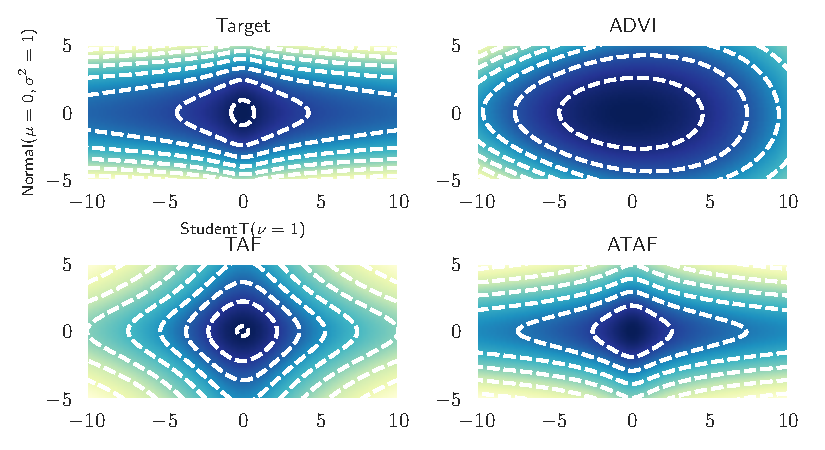
\includegraphics{../Figures/pancake.pdf}
    \vspace{-3mm}
  \caption{
    Variational inference against a tail-anisotropic target distribution $\cN(0,1) \otimes \text{StudentT}(\nu=1)$ (top left).
    Only ATAF (bottom right) is able to correctly reproduce the tail-anisotropy (fat-tailed along $x$-axis,
    Gaussian along $y$-axis).
    In contrast, ADVI's (top right) Gaussian base distribution and TAF's (bottom left) tail-isotropic $\prod_{i=1}^2 \text{StudentT}(\nu)$
    base distribution  can only model tail-isotropic distributions (\Cref{prop:isotropic-pushforward})
    which erroneously imposes power-law tails with the same rate of decay along both the $x$ and $y$ axes.
    \vspace{-5mm}
  }
  \label{fig:pancake}
\end{figure}

Our work here aims to address these deficiencies.
To understand the impact of the base distribution $\mu$ in flow-based models,
we develop and apply theory for fat-tailed random variables and their transformations under Lipschitz-continuous functions.
Our approach leverages the theory of concentration functions \citep[Chapter 1.2]{ledoux2001concentration} to significantly sharpen and extend prior results
\citep[Theorem 4]{jaini2019sum} by precisely describing the tail parameters of the pushforward distribution $(f_\theta)_\ast \mu$ under both Lipschitz-continuous (\Cref{thm:distn_class_closed}) and polynomial (\Cref{corr:closure_polynomials}) transport maps.
% \michael{We say ``characterize'' but what do we mean.  Probably this is the place to say that it is particularly important to be flexible to have different tail indices in different directions.  Then some of the later sentences will make sense.}
%In the multivariate setting, we observe that it is important to be flexible and allow for a multivariate distribution
%to have different tail parameters in different directions. %Accordingly,
In the multivariate setting,
we develop a theory of direction-dependent tail parameters (\Cref{def:mv-tail-param}), and show that tail-isotropic base distributions yield tail-isotropic pushforward measures (\Cref{prop:isotropic-pushforward}). 
As a consequence of \Cref{prop:isotropic-pushforward}, prior methods \citep{jaini2020tails} are limited in that
they are unable to capture \emph{tail-anisotropy}.
This motivates our development of \emph{anisotropic tail adaptive flows} (ATAF, \Cref{def:ataf}) as a means to
alleviate this issue (\Cref{remark:anisotropic}) and improve modeling of tail-anisotropic distributions.
% \michael{What limitation is precisely being referred to, since in the previous sentence we say that we get several results in this paper, and then we say how our results are a limitation.  Probably the best way to do this is to be more detailed, e.g., say that our \Cref{prop:isotropic-pushforward} means that the mapping can't introduce anisotropy.}
Our experiments show ATAF yields significant improvements in synthetic target distributions exhibiting fat-tails (\Cref{fig:cauchy_normal_student}) and tail-anisotropy (\Cref{fig:pancake}).
On realistic targets,
% prior work \citep[Table 2]{jaini2020tails} showed tail-adaptive flows (TAF, a subset of ATAF)
% can improve density modeling and 
We find (\Cref{sec:experiments}) that ATAF can yield significant improvements when applied for variational inference (VI).
% \michael{That sentence sounds like we are a footnote on them.  I would say that we get results for a ragne of cases, both for isotropic and anisotropic cases, thereby improving prior work that considered Gaussian things as well as prior work from \cite{jaini2020tails} that considered isotropic HT.}
\vspace{-3mm}
\subsection*{Related Work}
\vspace{-1mm}
\paragraph{Fat-tails in variational inference}

% The bulk of related work focuses on fat-tails arising from relaxing priors.
Recent work in variational autoencoders (VAEs) have considered relaxing Gaussian assumptions to heavier-tailed distributions \citep{mathieu2019disentangling,chen2019residual,boenninghoff2020variational,abiri2020variational}.
In \citep{mathieu2019disentangling}, a StudentT prior distribution $p(z)$ is considered over the latent code
$z$ in a VAE with Gaussian encoder $q(z \mid x)$, arguing
%\footnote{\url{https://github.com/iffsid/disentangling-disentanglement/blob/3396d40f46c34dd928a1241f567a86276b0ff41b/src/main.py\#L52}},
that the anisotropy of a StudentT product distribution leads to more disentangled representations as compared to the standard choice of Normal distributions.
A similar modification is performed in \cite{chen2020use}, for
a coupled VAE (see \cite{cao2019coupled}). It showed improvements in the marginal
likelihoods of reconstructed images. In addition,
\cite{boenninghoff2020variational} consider a mixture of StudentTs for the
prior $p(z)$. To position
our work in context, note that the encoder $q(z \mid x)$ may be viewed
as a variational approximation to the posterior $p(z \mid x)$ defined by the
decoder model $p(x \mid z)$ and the prior $p(z)$. Our work differs from
\citep{mathieu2019disentangling,chen2020use,boenninghoff2020variational} in
that we consider fat-tailed variational approximations $q(z \mid x)$ rather
than priors $p(z)$. Although \citep{abiri2020variational} also considers
a StudentT approximate posterior, our work involves a more general
variational family which use normalizing flows.
% Relaxation of priors to heavy-tailed distributions has numerous
% applications beyond VAEs. In \cite{silnova2018fast}, the authors perform
% inference in heavy-tailed probabilistic linear discriminant analysis
% using Gaussian mean-field variational inference and show improved
% accuracy in speaker identification. Our work is complementary to these approaches;
% whereas they consider heavy-tailed priors $p(z)$ we consider heavy-tailed
% variational families $q(z \mid x)$.
Similarly, although \citep{wang2018variational} also deals with fat-tails in variational inference,
their goal is to improve $\alpha$-divergence VI by controlling the moments of importance
sampling ratios (which may be heavy-tailed). Our work here adopts
Kullback-Leibler divergence and is concerned with enriching the variational family
to include anisotropic fat-tailed distributions.
More directly comparable recent work \cite{ding2011t,futami2017expectation} studies the $t$-exponential family
variational approximation which includes StudentTs and other
heavier-tailed densities. Critically, these do
not discuss selection of the parameter $t$ (which is deterministically to the
Student-T's DoF $\nu$), nor do they address the issue of tail anisotropy. %Other differences include their derivation of
%expectation-propagation update equations while 
% We directly backpropagate a noisy
% ELBO estimate, and introduce a richer variational family used by ATAF.

\vspace{-1mm}
\paragraph{Flow based methods}

Normalizing flows and other flow based methods have a rich history within variational
inference \citep{kingma2016improved,rezende2015variational,agrawal2020advances,webb2019improving}.
Consistent with our experience (\Cref{fig:blr-anisotropic}), \citep{webb2019improving}
documents normalizing flows can offer improvements over ADVI and NUTS across thirteen different
Bayesian linear regression models from \citep{gelman2006data}.
\citep{agrawal2020advances} shows that normalizing flows compose nicely with other
advances in black-box VI (e.g., stick the landing, importance weighting).
However, none of these works treat the issue of fat-tailed targets and inappropriate tail
decay.
To our knowledge, only TAFs \citep{jaini2020tails} explicitly consider flows with tails
heavier than Gaussians. Our work here can be viewed as a direct improvement of \citep{jaini2020tails},
and we make extensive comparison to this work throughout the body of this paper. At
a high level, we provide a theory for fat-tails which is sensitive to the rate of
tail decay and develop a framework to characterize and address the tail-isotropic limitations plaguing
TAFs.

\vspace{-2mm}
\section{Flow-based methods for fat-tailed variational inference}

%Continuing from the notation introduced in \Cref{sec:intro}, in this section we
%finish establishing the VI setting and definitions/notation
%\michael{I'm not sure what ``Continuing ...'' means.  Can we say ``In this section we do such-and such ...".  Maybe something like:
%``In this section, we provide background on flow-vased methods for VI, and we describe some of the issues that arise when dealing with fat-tailed data and fat-tailed VI that will be important for understanding our main results. 
%}

\vspace{-2mm}
\subsection{Flow-based VI methods} 

The objective of VI is to approximate a target distribution $\pi(x)$ by searching over
a \emph{variational family} $\cQ = \{q_\phi : \phi \in \Phi\}$ of probability distributions $q_\phi$.
While alternatives exist \citep{li2016variational,wang2018variational}, VI typically
seeks to find $q_\phi$ ``close'' to $\pi$ as measured by Kullback-Leibler divergence $\infdiv{q_\phi}{\pi}$.
To ensure tractability without sacrificing generality, in practice \citep{wingate2013automated,ranganath2014black}
a Monte-Carlo approximation of the evidence lower bound (ELBO) is maximized:
\begin{align*}
  %-\infdiv{q_\phi}{\pi}
  %\propto 
  \text{ELBO}(\phi)
  = \int q_\phi(x) \log \frac{\bar\pi(x)}{q_\phi(x)} dx
   & \approx \frac{1}{n} \sum_{i=1}^n \log \frac{\bar\pi(x_i)}{q_\phi(x_i)},
   && x_i \simiid q_\phi,
   && \bar{\pi} \propto \pi  .
\end{align*}
To summarize, this procedure enables tractable black-box VI
by replacing $\pi$ with $\bar\pi \propto \pi$ and approximating expectations with respect to $q_\phi$ (which are tractable only in simple variational families) through Monte-Carlo approximation. In Bayesian inference and probabilistic programming applications, the target posterior
$\pi(x) = p(x \mid y) = \frac{p(x, y)}{p(y)}$ is typically intractable but
$\bar\pi(x) = p(x,y)$ is computable (i.e. represented by the probabilistic program's
generative / forward execution).


\begin{table}
  \centering
  \begin{tabular}{ccc}
    \toprule
    Model                                  & Autoregressive transform                                                                              & Suff. conditions for Lipschitz         \\
    \midrule
    NICE\citep{dinh2014nice}               & $z_j + \mu_j \cdot \mathds{1}_{k \not \in [j]}$                                                       & $\mu_j$ Lipschitz                      \\
    MAF\citep{papamakarios2017masked}      & $\sigma_j z_j + (1 - \sigma_j) \mu_j$                                                                 & $\sigma_j$ bounded                     \\
    IAF\citep{kingma2016improved}          & $z_j \cdot \exp(\lambda_j) + \mu_j$                                                                   & $\lambda_j$ bounded, $\mu_j$ Lipschitz \\
    Real-NVP\citep{dinh2016density}        & $\exp(\lambda_j \cdot \mathds{1}_{k \not\in[j]}) \cdot z_j + \mu_j \cdot \mathds{1}_{k \not \in [j]}$ & $\lambda_j$ bounded, $\mu_j$ Lipschitz \\
    Glow\citep{kingma2018glow}             & $\sigma_j \cdot z_j + \mu_j \cdot \mathds{1}_{k \not\in [j]}$                                         & $\sigma_j$ bounded, $\mu_j$ Lipschitz  \\
    NAF\citep{huang2018neural}             & $\sigma^{-1}(w^\top \cdot \sigma(\sigma_j z_j + \mu_j))$                                              & Always \par (logistic mixture CDF)          \\
    NSF\citep{durkan2019neural}            & $z_j \mathds{1}_{z_j \not\in [-B,B]} + M_j(z_j;z_{<j}) \mathds{1}_{x_j \in [-B,B]}$         & Always \par (linear outside $[-B,B]$)     \\
    FFJORD\citep{grathwohl2018ffjord} & n/a (not autoregressive)                                                                              & Always \par (required for invertibility)    \\
    ResFlow\citep{chen2019residual} & n/a (not autoregressive)                                                                              & Always \par (required for invertibility)    \\
    \bottomrule
  \end{tabular}
  \caption{Some popular / recently developed flows, the autoregressive transform used in the flow (if applicable),
  and sufficient conditions conditions for Lipschitz-continuity. A subset of this table was first presented
  in \citep{jaini2020tails}. $M(\cdot)$ denotes monotonic rational quadratic splines \citep{durkan2019neural}.}
  \label{tab:flows}
\end{table}


While it is possible to construct a variational family $\cQ$ tailored to a specific task, we are interested in VI methods which are more broadly applicable and convenient to use: $\cQ$ should be automatically constructed from introspection of a given probabilistic model/program.
Automatic differentiation variational inference (ADVI) \citep{kucukelbir2017automatic} is an early implementation of automatic VI and it is still the default in certain probabilistic programming languages \citep{carpenter2017stan}.
ADVI uses a Gaussian base distribution $\mu$ and a transport map $f_\theta = f \circ \Phi_\text{Affine}$ comprised of an invertible affine transform composed with a deterministic transformation $f$ from $\RR$ to the target distribution's support (e.g., $\exp : \RR \to \RR_{\geq 0}$, $\text{sigmoid} : \RR \to [0,1]$).
As Gaussians are closed under affine transformations, ADVI's representational capacity is limited to deterministic transformations of Gaussians. Hence it cannot represent complex multi-modal distributions.
To address this, more recent work \citep{kingma2016improved,webb2019improving} replaces the affine map $\Phi_\text{Affine}$ with a flow $\Phi_{\text{Flow}}$ typically parameterized by an invertible neural network:
\begin{definition}
    \label[definition]{def:advi}
  ADVI (with normalizing flows) comprise the variational family
  $\cQ_\text{ADVI}~\coloneqq~\{
    (f~\circ~\Phi_\text{Flow})_\ast \mu
    \}$ 
  where $\mu = \text{Normal}(0_d, I_d)$,
  $\Phi_\text{Flow}$ is an invertible flow transform (e.g., \Cref{tab:flows})
  and $f$ is a deterministic bijection between constrained supports \citep{kucukelbir2017automatic}.
\end{definition}


As first noted in \citep{jaini2020tails}, the pushforward of a light-tailed Gaussian base distribution under a Lipschitz-continuous flow will remain light-tailed and provide poor approximation to fat-tailed targets. 
Despite this, 
%at the time of writing this paper 
many major probabilistic programming packages still make a default choice of Gaussian base distribution (\texttt{AutoNormalizingFlow}/\texttt{AutoIAFNormal} in Pyro \citep{bingham2019pyro}, \texttt{method=variational} in Stan \citep{carpenter2017stan}, \texttt{NormalizingFlowGroup} in PyMC \citep{patil2010pymc}).
%\michael{What is the verb in the following sentence}
To address this issue, tail-adaptive flows \citep{jaini2020tails} use a
base distribution $\mu_\nu = \prod_{i=1}^d \text{StudentT}(\nu)$
where a single degrees-of-freedom $\nu \in \RR$ is used across all $d$ dimensions. More precisely,
\begin{definition}
  \label[definition]{def:taf}
  Tail adaptive flows (TAF) comprise the variational family
  $\cQ_\text{TAF}
    \coloneqq \{
    (f \circ \Phi_\text{Flow})_\ast \mu_\nu
    \}$
  where $\mu_\nu = \prod_{i=1}^d \text{StudentT}(\nu)$ with $\nu$ shared across all $d$ dimensions
  and $f$ is a bijection between constrained supports \citep{kucukelbir2017automatic}.
  During training, the shared degrees of freedom $\nu$ is treated as an additional variational parameter.
\end{definition}


\vspace{-2mm}
\subsection{Fat-tailed variational inference}

\vspace{-1mm}
Fat-tailed variational inference (FTVI)
% \michael{I'm inclined to say that we should have ``(FTVI)'' and then refer to that acronym everywhere; then we can say: VI is important, FTVI is very important, ADVI did a good job with FTVI, we do a great job with FTVI, and you the reader should follow up on us and do FTVI.  It's the sort of acronym that is nice to remember.}
% will do, and add this discussion to future directions in conclusion
considers the setting where the target $\pi(x)$ is fat-tailed. 
Such distributions commonly arise during a standard
``robustification'' approach where light-tailed noise distributions are
replaced with fat-tailed ones \cite{tipping2005variational}. They also
appear when weakly informative prior distributions are used in Bayesian
hierarchical models \cite{gelman2006prior}.




To formalize these notions of fat-tailed versus light-tailed distributions, a quantitative classification for tails is required.
While prior work classified distribution tails according to quantiles and the existence of moment generating functions
\citep[Section 3]{jaini2020tails}, here we propose a more natural and finer-grained classification based upon
the theory of concentration functions \citep[Chapter 1.2]{ledoux2001concentration} which is sensitive to
the rate of tail decay.

\begin{definition}[Classification of tails]
    \label[definition]{def:tail-classification}
    For each $\alpha,p > 0$, we let 
    \vspace{-1mm}
    \begin{itemize}[leftmargin=*]
        \item $\mathcal{E}_\alpha^p$ denote the set of \emph{exponential-type} random variables $X$ with $\mathbb{P}(|X| \geq x) = \Theta(e^{-\alpha x^p})$;
    \vspace{-1mm}
        \item $\mathcal{L}_\alpha^p$ denote the set of \emph{logarithmic-type} random variables $X$ with $\mathbb{P}(|X| \geq x) = \Theta(e^{-\alpha(\log x)^p})$.
    \end{itemize}
    \vspace{-1mm}
    % A random variable $X$ is of %\textbf{exponential-type}, denoted $X \in \cE_\alpha^p$, w
    % \begin{description}
    %     \item[exponential-type], denoted $X \in \cE_\alpha^p$,
    %   whenever $\PP(\lvert X \rvert \geq x) = \Theta(e^{-\alpha x^p})$, and
    %     \item[logarithmic-type], denoted $X \in \cL^p_\alpha$, whenever $\PP(\lvert X \rvert \geq x) = \Theta(e^{-\alpha (\log x)^p})$.
    % \end{description}
    In both cases, we call $p$ the \emph{class index} and $\alpha$ the \emph{tail parameter} for $X$.
    Note that every $\cE_\alpha^p$ and $\cL_\beta^q$ are disjoint, that is,
    $\cE_\alpha^p \cap \cL_\beta^q = \emptyset$ for all $\alpha,\beta,p,q > 0$.
    For brevity, we define the ascending families
    $\overline{\cE_\alpha^p}$ and $\overline{\cL_\alpha^p}$
    analogously as before except with $\Theta(\cdot)$ replaced
    by $\cO(\cdot)$. Similarly, we denote the class of distributions with exponential-type
    tails with class index at least $p$
    by $\overline{\cE^p} = \cup_{\alpha \in \RR_+} \overline{\cE_\alpha^p}$, and similarly for $\overline{\cL^p}$.
\end{definition}

\begin{figure}[htbp]
  \centering
  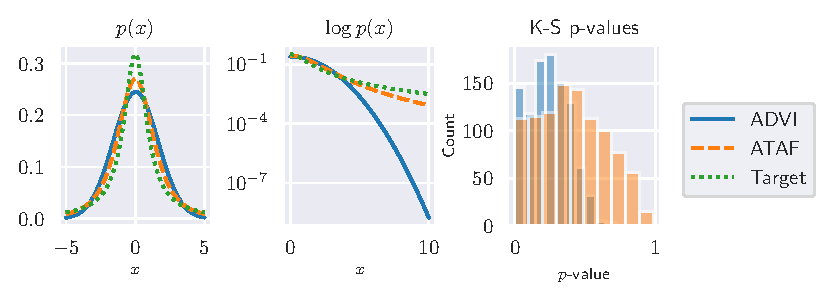
\includegraphics{../Figures/fat_tail_ks.pdf}
  \vspace{-6mm}
  \caption{
    When performing FTVI to approximate a $X \sim \text{Cauchy}(x_0 = 0, \gamma = 1)$ target (left panel, green dotted line),
    the use of a sub-Gaussian variational family (ADVI, solid blue line) can incur
    exponentially bad tail approximations (middle panel) compared to
    methods which permit heavier tails (ATAF, green dashed line) and results in
    samples which are more similar to the target (as measured by $1000$ repeats of
    1-sample $N=100$ Kolmogorov-Smirnov $p$-values, right panel).
    % \michael{Why does (b) look so good; are the tails really perfect, of if we went out to 15 or 30 on the X axis.  It might be good to show ATAF is much better but still not perfect.  Also, what is the X axis on each figure.  }
    % \feynman{updated the figure, hope it addresses the comment!}
  }
  \label{fig:cauchy_normal_student}
\end{figure}

For example, $\overline{\cE_\alpha^2}$ corresponds to $\alpha^{-1/2}$-sub-Gaussian random variables,
    $\overline{\cE_\alpha^1}$ corresponds to sub-exponentials, and (of particular relevance to this paper) $\cL^1_\alpha$ corresponds to the class of power-law distributions.
The motivation for the fat-tailed variational families used in TAF/ATAF
is easily illustrated on a toy example consisting of $X \sim \text{Cauchy}(x_0 = 0, \gamma = 1) \in \cL^1_1$.
As seen in \Cref{fig:cauchy_normal_student}, while ADVI with normalizing flows \citep{kingma2016improved,webb2019improving}
appears to provide a reasonable fit to the bulk of the target distribution (left panel), the improper
imposition of sub-Gaussian tails results in an exponentially bad tail approximation (middle panel).
As a result, samples drawn from the variational approximation fail a Kolmogorov-Smirnov goodness-of-fit
test against the true target distribution much more often (right panel, smaller $p$-values imply more rejections)
than a variational approximation which permits fat-tails. This example is a special case of \Cref{thm:distn_class_closed}.

\vspace{-2mm}
\section{Tail behavior of Lipschitz flows}

\vspace{-1mm}
This section states our main theoretical contributions; proofs are deferred to \Cref{sec:proofs}.
We sharpen previous impossibility results approximating fat-tailed targets
using thin-tailed base distributions \citep[Theorem 4]{jaini2020tails}
by characterizing the effects of Lipschitz-continuous transport maps on not only the tail class
but also the class index and tail parameter (\Cref{def:tail-classification}). Furthermore, we extend the theory
to include polynomial flows \cite{jaini2019sum}. For the multivariate setting,
we define the tail-parameter function (\Cref{def:mv-tail-param}) to help formalize the notion
of tail-isotropic distributions and prove a fundamental limitation that tail-isotropic
pushforwards remain tail-isotropic (\Cref{prop:isotropic-pushforward}).

Most of our results are developed within the context of Lipschitz-continuous transport maps $f_\theta$.
In practice, many flow-based methods exhibit Lipschitz-continuity in their transport map either by design \citep{grathwohl2018ffjord,chen2019residual}, or as a consequence of choice of architecture and activation function (\Cref{tab:flows}). % or by being enforced stemming from the Banach fixed point theorem 
%
%or .
The following assumption encapsulates this premise.
\begin{assumption}\label[assumption]{assump:lipschitz}
    $f_\theta$ is Lipschitz continuous (e.g., sufficient conditions in \Cref{tab:flows} are satisfied) and invertible.
\end{assumption}


\vspace{-2mm}
\subsection{Closure of tail classes}
\label{ssec:failure}

\vspace{-1mm}
Our first set of results pertain to closure of the tail classes in \Cref{def:tail-classification}
under Lipschitz-continuous transport maps. While earlier work \citep{jaini2020tails} demonstrated
closure of exponential-type distributions $\cup_{p > 0} \overline{\cE^p}$ under flows satisfying \Cref{assump:lipschitz}, our results in Theorem \ref{thm:distn_class_closed}, and Corollaries \ref{corr:heavy_to_light} and \ref{corr:closure_polynomials} sharpen these observations, showing that (1) Lipschitz transport maps cannot decrease the class index $p$ for exponential-type random variables, but can alter the tail parameter $\alpha$; and
(2) under additional assumptions, cannot change either class index $p$ or the tail parameter $\alpha$ for logarithmic-type random variables.
%         tail parameter $\alpha$; 
% \begin{itemize}[leftmargin=*]
%     \item cannot decrease the class index $p$ for exponential-type random variables, but can alter the
%         tail parameter $\alpha$; and
%     \item under additional assumptions, cannot change either class index $p$ or the tail
%         parameter $\alpha$ for logarithmic-type random variables.
% \end{itemize}

\begin{theorem}[Lipschitz maps of tail classes]
  \label{thm:distn_class_closed}
  Under \Cref{assump:lipschitz},
  the distribution classes $\overline{\cE^p}$
  and $\overline{\cL^p_\alpha}$ (with $p,\alpha > 0$) are closed
  under every flow transformation in \Cref{tab:flows}.
\end{theorem}

Informally, \Cref{thm:distn_class_closed} asserts that light-tailed base distributions cannot be transformed
via Lipschitz transport maps into fat-tailed target distributions.
Note this does not violate universality theorems for certain flows \cite{huang2018neural}
as these results only apply in the infinite-dimensional limit. Indeed, certain exponential-type families (such as Gaussian mixtures) are dense in the class of \emph{all} distributions, including those that are fat-tailed.

Note that $\overline{\cL^p_\alpha} \supset \cE^q_\beta$ for all $p,q,\alpha,\beta$, so \Cref{thm:distn_class_closed}
by itself does not preclude transformations of fat-tailed base distributions to light-tailed targets.
Under additional assumptions on $f_\theta$, we further establish a partial converse that a fat-tailed base distribution's tail parameter is unaffected after pushfoward
hence heavy-to-light transformations are impossible. Note here there is no ascending union over
tail parameters (i.e., $\cL^p_\alpha$ instead of $\overline{\cL^p_\alpha}$).

\begin{corollary}[Closure of $\cL^p_\alpha$]
  \label[corollary]{corr:heavy_to_light}
  If in addition $f_\theta$ is smooth
  with no critical points on the interior or boundary of
  its domain, then $\cL_\alpha^p$ is closed.
\end{corollary}

This implies that simply fixing a fat-tailed base
distribution \emph{a priori} is insufficient; the tail-parameter(s) of the base distribution must be explicitly optimized alongside
the other variational parameters during training.
While these additional assumptions may seem restrictive, note that many flow transforms
explicitly enforce smoothness and monotonicity \citep{wehenkel2019unconstrained,huang2018neural,durkan2019neural}
and hence satisfy the premises. In fact, we can show a version of \Cref{thm:distn_class_closed} ensuring closure of exponential-type
distributions under polynomial transport maps which do not satisfy \Cref{assump:lipschitz}.
This is significant because it extends the closure results to
include polynomial flows such as sum-of-squares flows \citep{jaini2019sum}.

\begin{corollary}[Closure under polynomial maps]
    \label[corollary]{corr:closure_polynomials}
  For any $\alpha, \beta, p, q \in \RR_+$, there does not exist a
  finite-degree polynomial map from $\cE_\alpha^p$ into $\cL_\beta^q$.
\end{corollary}

% Suffices to show for k \in \RR_{> 0}, this covers inverse powers

% \begin{remark}
%   There does not exist a inverse polynomial map (e.g., sqrt) from $\cL_\alpha$ to $\cE$.
% \end{remark}

\vspace{-2mm}
\subsection{Multivariate fat-tails and anisotropic tail adaptive flows}

\vspace{-1mm}
Next, we develop theory for fat-tailed random elements in the multivariate setting which leads to formalized notions of isotropic/anisotropic tail indices. Using our theory, we prove that both ADVI and TAF are fundamentally limited because they
are only capable of fitting tail-isotropic target measures (\Cref{prop:isotropic-pushforward}).
To address this limitation, we propose anisotropic tail adaptive flows (ATAF) as a density
modeling method which can represent tail-anisotropic distributions (\Cref{remark:anisotropic}).

% Karamata's theorem enables recovery of a regularly varying random variable's
% index: $X \in \cL^1_\alpha$ means that $\lim_{x \to \infty} \frac{x \PP(X \geq
%     x)}{\int_x^\infty \PP(X \geq t) dt} = \alpha$ for $\alpha < -1$.
% Motivated by Karamata's theorem, we introduce
% the following definition to aid in describing multivariate fat-tailed random variables:

For example, consider the target distribution shown earlier in \Cref{fig:pancake} formed as the product of $\mathcal{N}(0,1)$ and $\text{StudentT}(\nu=1)$ distributions.
The marginal/conditional distribution along a horizontal slice (e.g., the distribution of $\braket{X,e_0}$)
is fat-tailed, while along a vertical slice (e.g., $\braket{X,e_1}$) it is Gaussian.
Another extreme example of tail-anisotropy where the tail parameter for
$\braket{X,v}$ is different in every direction $v \in \cS^{1}$
is given in \Cref{fig:radial-fat-tail}. Here $\mathcal{S}^{d-1}$ denotes the $(d-1)$-sphere in $d$ dimensions. 
Noting that the tail parameter depends on the choice of direction, we are motivated to consider
the following direction-dependent definition of multivariate tail parameters. 

\begin{definition}
  \label[definition]{def:mv-tail-param}
  For a $d$-dimensional random vector $X$,
  its \emph{tail parameter function} $\alpha_X : \cS^{d-1} \to \bar{\RR}_+$
  is defined as
  % $\alpha_X(v) = \lim_{x \to \infty} \frac{x \PP(\braket{v,X} \geq x)}{\int_x^\infty \PP(\braket{v,X} \geq t) dt}$.
  $\alpha_X(v) = \lim_{x \to \infty} \frac{\log \PP(\braket{v,X} \geq x)}{\log x}$ when the limit exists, and $\alpha_X(v) = +\infty$ otherwise.
  In other words, $\alpha_X(v)$ maps directions $v$ into the tail index of the corresponding one-dimensional projection $\braket{v,X}$. The random vector $X$ is \emph{tail-isotropic} if $\alpha_X(v) \equiv c$ is constant. Otherwise, it is \emph{tail-anisotropic}. 
\end{definition}


\begin{figure}[htbp]
  \centering
  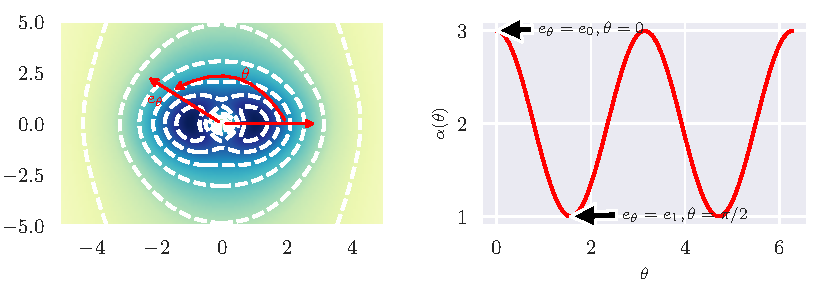
\includegraphics{../Figures/radial-fat-tail.pdf}%
  %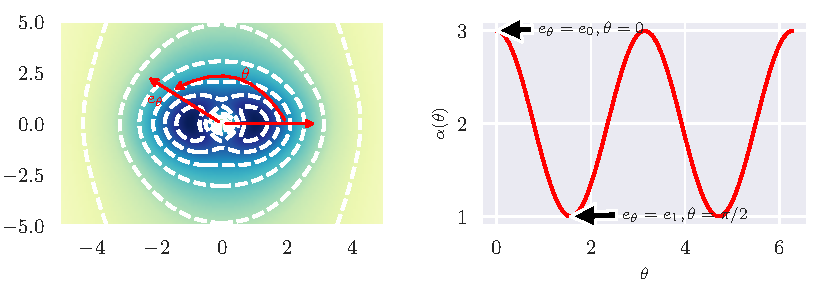
\includegraphics[width=\textwidth]{../Figures/radial-fat-tail.png}%
  %\input{../Figures/radial-fat-tail.pgf}
  \vspace{-3mm}
  \caption{
    Illustration of the direction-dependent tail-parameter function (right) on a tail-anisotropic distribution (left)
    with PDF $\dd P(r,\theta) = r^{-\alpha(\theta)} r \dd r \dd\theta$ and tail parameter $\alpha(\theta) = 2 + \cos(2\theta)$.
    While prior fat-tailed theory based on $\|X\|_2 = \sup_{\|v\|_2 = 1} \braket{X,v}$
    is only sensitive to the largest tail parameter $\max_{\theta \in [0, 2\pi]} \alpha(\theta) = 3.0$,
    our direction-dependent tail parameter function (right, red line)
    and its values along the standard basis axes ($\alpha(0)$ and $\alpha(\pi/2)$)
    capture \emph{tail-anisotropy}.
  }
  \label{fig:radial-fat-tail}
\end{figure}
% \begin{definition}
%   \label[definition]{def:isotropic}
%   Multivarate random variable $X$ is tail-isotropic if $\alpha_X(v) \equiv c$ is constant.
%   Otherwise, it is tail-anisotropic.
% \end{definition}


% \begin{align*}
%   \PP[\braket{X,u} \geq x]
%   = \PP[\braket{\mu,u} + R \braket{AU,u} \geq x]
%   = \PP[R \geq \frac{x - \braket{\mu,u}}{\braket{u,AU}}]
%   \sim C_1 \left(\frac{x - \braket{\mu,u}}{\braket{u,AU}}\right)^{-\alpha}
%   \sim C_2 x^{-\alpha}
% \end{align*}
% and
% theory around tail parameters is developed for elliptically
% contoured multivariate distributions $X = \mu + R A U$
% for some heavy-tailed random variable $R$, fixed vectors $\mu \in \RR^d$
% and $U \in S^{d-1}$, and $A$ a (Cholesky factor)
% defining the ellipsoid axes.

% While elliptically contoured multivariate distributions admit a
% straightforward generalization from the scalar case, they are severely
% limited in practical applications.  One fundamental limitation of
% elliptically contoured $X$ is that the tail parameter is the same for every
% 1-dimension projection.  If $R$ has tail index $\alpha$ then for all for $u
%   \in S^{d-1}$
% \begin{align*}
%   \PP[\braket{X,u} \geq x]
%   = \PP[\braket{\mu,u} + R \braket{AU,u} \geq x]
%   = \PP[R \geq \frac{x - \braket{\mu,u}}{\braket{u,AU}}]
%   \sim C_1 \left(\frac{x - \braket{\mu,u}}{\braket{u,AU}}\right)^{-\alpha}
%   \sim C_2 x^{-\alpha}
% \end{align*}

% Furthermore, the assumption of elliptical distributions are
% easily violated in many common and useful applications.  For example, in
% probabilistic programming collections of random variables are oftentimes
% grouped together into a single multivariate random variable (e.g.,  blocked
% Gibbs, Hamiltonian Monte Carlo).  In fact, $Q_{TAF}$ (used in the experiments
% in \citep{jaini2020tails}) uses a StudentT product base distribution which
% is not elliptically symmetric.

% \begin{figure}[htbp]
%   \centering
%   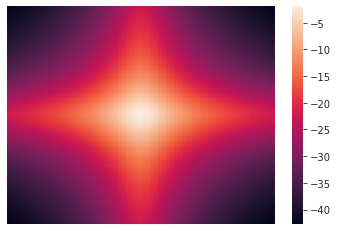
\includegraphics[width=0.4\textwidth]{../Figures/studentt-product.png}
%   \caption{
%     Illustrating multivariate fat-tails using a 2-dimensional StudentT.
%     The multivariate theory from \citep{jaini2020tails} is for elliptically
%     contoured distributions and not applicable to the StudentT product base distributions
%     used in their experiments.
%   }
%   \feynman{Consider just using words here to delineate from our contributions, this is not a super important fact}
%   \label{fig:studentt-product}
% \end{figure}




% Elliptical distributions are \emph{tail isotropic} i.e., $\alpha(v) \equiv c$ is constant.
% The base distribution for \citep{jaini2020tails}, $\prod_1^d \text{StudentT}(\nu_i)$ with $\nu_i \equiv \nu$,
% is also tail isotropic because
% $\braket{v,X}$ is a sum of StudentT and by tail index algebra
% has index $\max_i \nu_i = \nu$.

It is illustrative to contrast this to the theory presented for TAF \citep{jaini2020tails}
where only the tail exponent of $\|X\|_2$ is considered.
For $X = (X_1, \ldots, X_d)$ with $X_i \in \cL^1_{\alpha_i}$, 
\begin{align*}
  \PP[\|X\|_2 \geq t]
  = \PP\left[\sup_{v \in \cS^{d-1}} \braket{X,v} \geq t\right]
  \geq \sup_{v \in \cS^{d-1}} \PP[\braket{X,v} \geq t]
  = \max_{1 \leq i \leq d} \nu_i
  = \max_{0 \leq i \leq d-1} \alpha_X(e_i).
\end{align*}
Therefore, considering only the tail exponent of $\|X\|_2$ is equivalent to summarizing $\alpha_X(\cdot)$ by an upper bound.
Given the absence of the tail parameters for other directions (i.e., $\alpha_X(v) \neq \sup_{\|v\|=1} \alpha_X(v)$)
in the theory for TAF \citep{jaini2020tails}, it should be unsurprising that both their multivariate 
theory as well as their experiments only consider tail-isotropic distributions obtained either
as an elliptically-contoured distribution with fat-tailed radial distribution or 
$\prod_{i=1}^d \text{StudentT}(\nu)$ (tail-isotropic by \Cref{lem:sum-rule}). 
Our next proposition shows that this presents a significant limitation when the target distribution is
tail-anisotropic.


\begin{proposition}[Pushforwards of tail-isotropic distributions]
  \label[proposition]{prop:isotropic-pushforward}
  Let $\mu$ be tail isotropic with index $\nu$.
  and suppose $f_\theta$ satisfies \Cref{assump:lipschitz}.
  Then $(f_\theta)_\ast \mu$ is tail isotropic with index $\nu$.
\end{proposition}

% However, $\alpha(v)$ is non-trivial to work with; it is an asymptotic quantity and is defined
% for uncountably many $v \in S^{d-1}$. In this work, we propose approximating
% $\alpha(v)$ using the standard basis vectors:

% \begin{definition}
%   The \emph{standard basis tail parameters} of a fat-tailed $X \in \RR^d$
%   is $\{\alpha(e_i) : i \in [d]\}$ where $\alpha$ is defined in
%   \Cref{def:mv-tail-param} and $e_i$ is the $i$th standard basis vector.
% \end{definition}

% The standard basis vectors provide a natural choice of projections for
% multivariate product distributions (as commonly encountered during blocking /
% grouping of random variables). Going back to our previous example,
% we still have that $\alpha_{\|X\|} = \max_i \alpha(e_i)$ but now the tail
% indices of the remaining $e_j$ need not be equal. Admittedly, the standard basis
% is less suitable for correlated multivariate distributions. For example,
% let $t_i \sim \text{StudentT}(\nu_i)$ and consider the rotated random variable
% $X = R_{\pi/4} [t_1; t_2]$. Its standard basis tail parameters are
% \begin{align*}
%   \Pr[\braket{X,e_1} > x]
%   = \Pr[\braket{X,e_2} > x]
%   = \Pr[0.5 t_1 + 0.5 t_2 > x]
%   \leq \max_i \nu_i
% \end{align*}
% This example illustrates that the standard basis tail parameters
% provide multivariate tail parameters which are no worse than
% previous work.

% \subsection{Limitations of our theory}

% \begin{itemize}
%   \item Standard basis parameters not general, only works for axis-aligned tails
%   i.e., independent product distributions
%   \item Still fails on the spiral, but it should do better than TAF
%   \item Theory not fully general, only considers rays from origin rather than
%   path integrals
% \end{itemize}

To work around this limitation without relaxing \Cref{assump:lipschitz}, it is evident
that tail-anisotropic base distributions $\mu$ must be considered. In this work, we propose
the following model which replaces TAF's isotropic base distribution $\prod_{i=1}^d \text{StudentT}(\nu)$
with $\prod_{i=1}^d \text{StudentT}(\nu_i)$. Note that $\nu$ is no longer shared across dimensions,
enabling $d$ different tail parameters to be represented:

\begin{definition}\label[definition]{def:ataf}
  Anisotropic Tail-Adaptive Flows (ATAF) comprise the variational family
  $\cQ_\text{ATAF}~\coloneqq~\{
    (f \circ \Phi_\text{Flow})_\ast \mu_\nu
    \},$
  where $\mu_\nu = \prod_{i=1}^d \text{StudentT}(\nu_i)$, each $\nu_i$ is \emph{distinct}, and $f$ is a bijection between constrained supports \citep{kucukelbir2017automatic}.
\end{definition}


\begin{remark}\label[remark]{remark:anisotropic}
  Anisotropic tail-adaptive flows can represent tail-anisotropic distributions with up to $d$ different
  tail parameters while simultaneously satisfying \Cref{assump:lipschitz}.
  For example, if $\Phi_\text{Flow} = \text{Identity}$ and $\mu_\nu = \prod_{i=1}^d \text{StudentT}(i)$
  then the pushforward $(\Phi_\text{Flow})_\ast \mu_\nu = \mu_\nu$ is tail-anisotropic.
  % Moreover, its standard basis tail parameters are equal
  % (up to permutation) to those for $\mu$.
\end{remark}

% Compared to \citep{jaini2020tails}, the degrees of freedom $\nu$ is no longer
% shared across all $d$ dimensions so the variational approximations may exhibit
% varying degrees of fat-tailedness across different dimensions. As seen in
% \Cref{fig:pancake}, such anisotropy is particularly important in situations
% such as the ``heavy-tailed pancake.'' This situation is particularly relevant in
% probabilistic programming, where multiple latent variariables (potentially of different
% tail index) are blocked together for joint sampling / approximation.

\vspace{-2mm}
\subsection{Discussion of limitations}
\label{ssec:limitations}

\vspace{-1mm}
Whereas the tail-parameter function $\alpha_X(\cdot)$ provides finer-grained characterization
of multivariate tails, it still possesses some notable limitations.
By only considering projections $\braket{X,v}$ along rays through the origin
$v \in \cS^{d-1}$ precludes situations where the limit in $\alpha_X(\cdot)$ is not well defined.
For example, consider $\text{StudentT}(\nu=1) \otimes \text{StudentT}(\nu=2)$ and ``spin'' it
using the radial transformation $(r,\theta) \mapsto (r,r+\theta)$ (\Cref{fig:spiral}). Due to
oscillations, $\alpha_X(v)$ is not well defined for all $v \in \cS^{1}$. 


\begin{figure}[htbp]
    \centering
    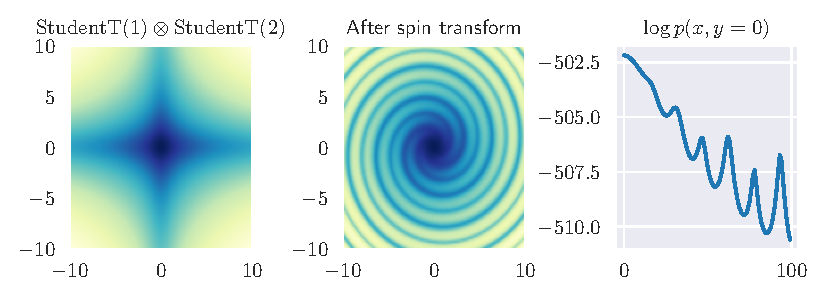
\includegraphics{Figures/spiral.pdf}
    \caption{Taking a tail-anisotropic distribution (left) and ``spinning'' it (middle) results in
        one-dimensional projections which oscillate between tail parameters (as seen in
        $\log p(\braket{X,e_0})$ in right panel) and cause $\alpha_X(\cdot)$ to be not well defined.
    }
    \label{fig:spiral}
\end{figure}

Additionally, note that ATAF only uses a finite collection $\{\nu_i\}_{i=1}^d$ of tail parameters
whereas the tail-parameter function may take on more than $d$ values. \Cref{fig:radial-fat-tail}
presents a worst-case scenario, where the target distribution has a continuum of tail parameters.
As ATAF is only capable of representing $d$ different tail parameters in its pushforward
(\Cref{remark:anisotropic}), it will necessarily incur an approximation error when $> d$ different
tail parameters are present.

While it is true that ATAF imposes logarithmic-type tails for all projections $\braket{X,v}$,
note that $\text{StudentT}(\nu) \Rightarrow \cN(0,1)$ as $\nu \to \infty$ so we should expect
ATAF to provide reasonably good approximations to target distributions in $\overline{\cE^2}$
by taking $\nu$ sufficiently large. We observed this occurs in practice empirically
in \Cref{sec:normal-normal-location-mixture}.
% We found that applying ATAF when the target is light tailed results in minimal
% error (\Cref{sec:normal-normal-location-mixture}); the result agrees with
% intuition because $\text{StudentT}(\nu) \to N(0,1)$ as $\nu \to \infty$ so
% it is reasonable to expect ATAF to learn reasonable approximations.

% \subsection{Non-parametric tail index estimation}
% \label{ssec:non-param-index}

% To perform variational inference with $\cQ_{ATAF}(\nu,\Phi)$, note that if
% $\Phi$ is Lipschitz then the tail index of any element of
% $\cQ_{ATAF}(\nu,\Phi)$ depends only on $\nu$. This motivates a two step
% procedure where (1) $\hat\nu$ estimates the degrees of freedom and
% (2) standard normalizing-flow variational inference $\max_\Phi \cQ_{ATAF}(\hat\nu,\Phi)$ is performed. The key advantage here is that both steps are standard,
% so existing techniques for tail index estimation may be applied.

% Let $X$ be a random variable with fat-tailed density $\pi(x)$
% with tail index $\alpha$ which we wish to estimate.
% When samples $X_i \simiid \pi$ are tractable
% (e.g., no \texttt{observe} or \texttt{condition} statements), traditional
% tail-index estimation techniques may be applied:

% \begin{figure}[H]
%   \centering
%   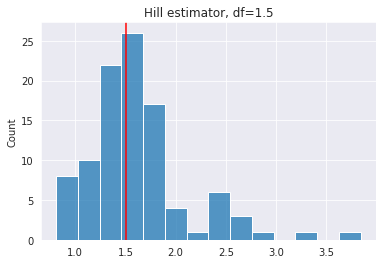
\includegraphics[width=0.6\textwidth]{../Figures/hill.png}
%   \caption{Hill estimator against $\nu=1.5$ StudentT}
%   \label{fig:hill}
% \end{figure}

% Oftentimes $\pi$ is the posterior distribution of latent variable $X$
% after conditioning on observations $Y=y$, in which case
% $\pi(x) = p(X=x \mid Y=y) = \frac{p(x,y)}{p(y)}$
% and sampling from $\pi$ is non-trivial.
% To circumvent this, we propose the following asymptotically correct
% estimator. Note for $a, b$ large:
% \begin{align*}
%   \Pr[X > a]                 & \sim b^{-\alpha}                                           \\
%   \pi(a)                     & \sim \alpha a^{-\alpha - 1}                                \\
%   \log \pi(a)                & \sim \log \alpha - (\alpha + 1) \log a                     \\
%   \log \frac{p(a,y)}{p(b,y)} & = \log \frac{\pi(a)}{\pi(b)}
%   \sim (\alpha + 1) \log \frac{b}{a}                                                      \\
%   \alpha                     & \sim \frac{\log p(a,y) - \log p(b,y)}{\log b - \log a} - 1
% \end{align*}
% The joint density $p(x,y)$ is tractably computed by running the
% probabilistic program forwards.
% For example. setting $a=10$ and $b=20$ yields an estimate of $1.4799$ for a
% $\nu=1.5$ StudentT.

% \subsubsection{Approximating 1D-marginals}

% This is an example of a two-point log-linear extrapolation at points $a$ and $b$.
% \feynman{Consider Richardson extrapolation to accelerate this limit. Rate of convergece in limit must be a power}

% In general, PPs may include several latent variables.
% The 1-dimensional marginal $p(x, y) = \int_{\setminus x} p(x,z,y) dz$
% is required to apply the above interpolation method.
% We propose approximating this integral using discrete samples.
% If $z$ is a descendent of $y$, then
% we can compute $p(x,y)$ by executing the probabilistic program
% (possibly terminating early).
% If $z$ is an ancestor of $x$ (hence also an ancestor of $y$), then
% \begin{align*}
%   p(x,y) \approx \frac{1}{N} \sum_{i=1}^N p(y, x \mid z_i)
%   \qquad z_i \simiid p(z)
% \end{align*}
% In the last case where $x \rightarrow z \rightarrow y$,
% we have
% \begin{align*}
%   p(x,y) \approx p(x) \frac{1}{N} \sum_{i=1}^n p(y \mid x, z_i)
%   \qquad z_i \simiid p(z_i \mid x)
% \end{align*}

% \begin{figure}[H]
%   \centering
%   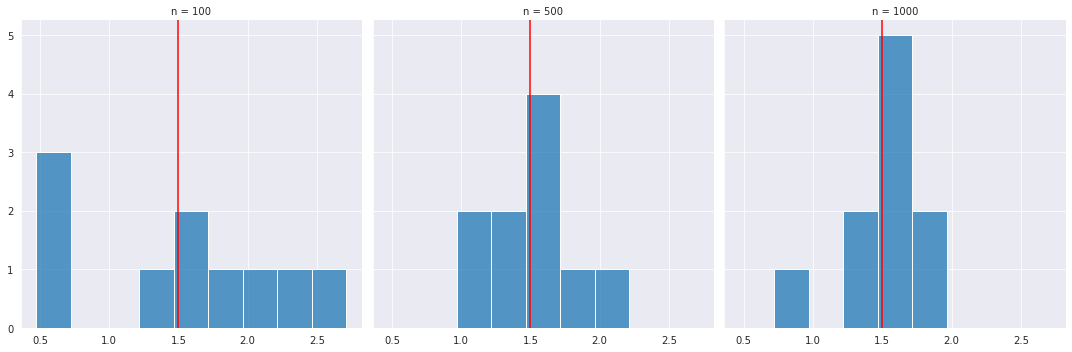
\includegraphics[width=0.9\textwidth]{../Figures/our-estimator.png}
%   \caption{Tail index estimation on location-scale mixture representation
%     for StudentT, where the mixture is discretized to $n$ components.}
%   \label{fig:approx_marg}
% \end{figure}

\vspace{-2mm}
\section{Experiments}
\label{sec:experiments}

\vspace{-1mm}
While previous sections demonstrated the improvements of ATAF on synthetic problems
exhibiting tail-anisotropy, in this section we validate ATAF's ability to improve
a range of probabilistic modeling tasks. As improvements in density
modeling using TAFs (a subset of ATAF) have already been shown in prior work \citep{jaini2020tails},
our experiments complement these results by focusing on VI tasks and demonstrating the
efficacy of ATAF.
Our experiments are implemented using the 
%\texttt{beanmachine} probabilistic programming language\citep{tehrani2020bean}
\texttt{REDACTED FOR REVIEW} probabilistic programming language[REDACTED]
and the
%\texttt{flowtorch} library for normalizing flows\citep{flowtorchai},
\texttt{REDACTED FOR REVIEW} library for normalizing flows[REDACTED],
%and we have open-sourced the code\citep{ghlic}
and we have open-sourced the code[REDACTED, reviewers please see supplementary materials for code]
under a CC-BY-NC license. Additional details for the experiments are detailed in \Cref{sec:additional-exp-details}.

% These experiments investigate the behavior of neural density estimators with
% \emph{heavy-tailed base distribution}.
% Specifically, we consider a masked autoregressive flow \cite{papamakarios2017masked}
% transform of a generalized Student's t distribution as a density estimator $q_\theta(X)$
% in a variational inference framework. To fit $q_\theta$ to a target distribution
% $\pi$, the ELBO gradient is reparameterized and Monte-Carlo approximated
% \begin{align*}
%   \nabla_\theta \EE_{q_\theta} \log \frac{\pi(X)}{q_\theta(X)}
%   & = \nabla_\theta \EE_p \log \frac{
%     \pi(X)
%   }{p_\theta(f_\theta^{-1}(X))
%   \left\lvert \det \nabla f_\theta^{-1}(X) \right\rvert}    \\
%   & = \EE_p \nabla_\theta \log \frac{
%     \pi(X)
%   }{p_\theta(f_\theta^{-1}(X))
%   \left\lvert \det \nabla f_\theta^{-1}(X) \right\rvert}    \\
%   & \approx \frac{1}{n} \sum_i^n \nabla_\theta \log \frac{
%     \pi(x_i)
%   }{p_\theta(f_\theta^{-1}(x_i))
%     \left\lvert \det \nabla f_\theta^{-1}(x_i) \right\rvert}
% \end{align*}


\subsection{Bayesian linear regression with conjugate priors}

For our first experiment, we consider one-dimensional Bayesian linear regression (BLR)
with conjugate priors. This model is defined by priors and likelihood
\begin{align*}
    \sigma^2 \sim \text{Inv-Gamma}(a_0, b_0), \qquad
    \beta \mid \sigma^2 \sim \cN(0, \sigma^2),\qquad 
    y \mid X, \beta, \sigma \sim \cN(X \beta, \sigma^2) 
\end{align*}
where $a_0$, $b_0$ are hyperparameters and the task is to approximate the posterior
distribution $p(\beta,\sigma^2 \mid X, y)$. Owing to conjugacy,
the posterior distribution can be explicitly computed. Indeed, $p(\beta,\sigma^2 \mid X, y) = \rho(\sigma^2)\rho(\beta \mid \sigma)$ where $\rho(\beta \mid \sigma) = \cN(\Sigma_n(X^\top X \hat\beta), \sigma^2 \Sigma_n)$, $\Sigma_n = (X^\top X + \sigma^{-2})^{-1}$, $\hat\beta = (X^\top X)^{-1} X^\top y$, and
%\begin{align*}
    %p(\beta,\sigma^2 \mid X, y) &= \rho(\sigma^2) \rho(\beta \mid \sigma) \\
    \[
    \rho(\sigma^2) = \text{Inv-Gamma}\bigg(
    %\underbrace{a_0 + \frac{n}{2}}_{\eqqcolon a_n}, 
    a_0 + \frac{n}{2}, 
    b_0 + \frac{1}{2}(y^\top y - \mu_n^\top \Sigma_n \mu_n)\bigg)% \\
    \]
    %\rho(\beta \mid \sigma) &= \cN(\Sigma_n(X^\top X \hat\beta), \sigma^2 (X^\top X + \sigma^{-2} I)^{-1})
%\end{align*}
This calculation reveals that the posterior distribution is tail-anisotropic:
for fixed $c$ we have that $p(\sigma^2, \beta=c \mid X, y) \propto \rho(\sigma^2) \in \cL^1_{\alpha_n}$
as a function of $\sigma$
and $p(\sigma^2=c, \beta \mid X, y) \propto \rho(\beta \mid c) \in \overline{\cE^2}$
as a function of $\beta$.
As a result of \Cref{prop:isotropic-pushforward}, we expect ADVI and TAF to erroneously impose
Gaussian and power-law tails respectively for both $\beta$ and $\sigma^2$ as neither method
can produce a tail-anisotropic pushforward. This intuition is confirmed in \Cref{fig:blr-anisotropic},
where we see that only ATAF is the only method capable of modeling the tail-anisotropy present.
 

\begin{figure}[htbp]
  \centering
  \vspace{-0.5cm}
  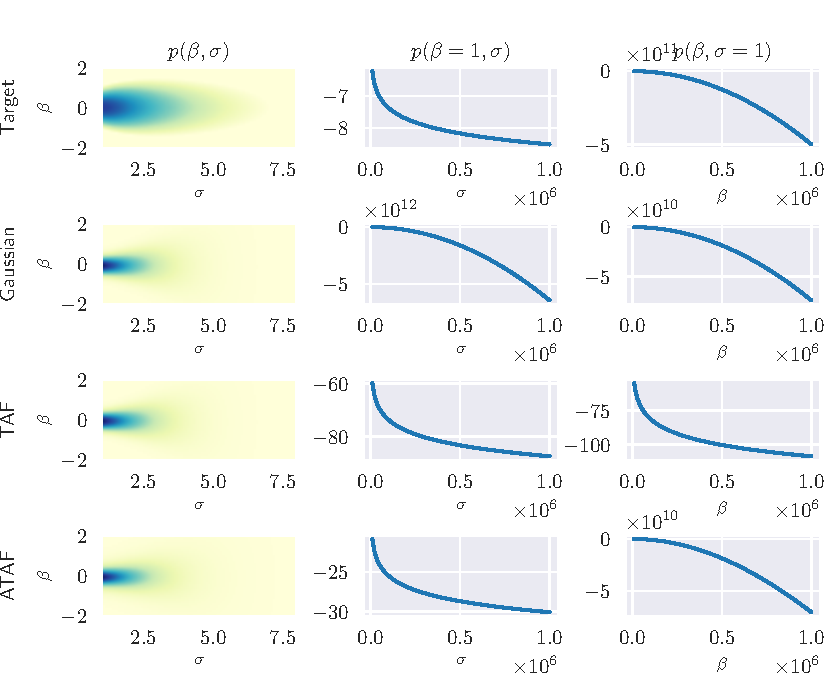
\includegraphics{../Figures/blr_aniso.pdf}
  \vspace{-0.5cm}
  \caption{
    Bayesian linear regression's tail-anisotropic posterior
    (top left) exhibits a fat-tailed conditional in $\sigma$ (as evidenced by
    the convex power-law decay in the top middle panel) and a Gaussian conditional in $\beta$ (concave graph in top right panel).
    While all methods appear to provide a good approximation of the bulk (left column),
    \Cref{prop:isotropic-pushforward} implies
    Gaussian (Gaussian, second row) or isotropic StudentT product (TAF, third row) base distribution
    yields Gaussian or power-law tails respectively for \emph{both} $\sigma$ and $\beta$.
    In contrast, ATAF (bottom row) illustrates \Cref{remark:anisotropic} by simultaneously
    modeling a power-law tail on $\sigma$ and Gaussian tail on $\beta$.
  }
  \label{fig:blr-anisotropic}
\end{figure}



\begin{table}[htbp]
  \centering
%   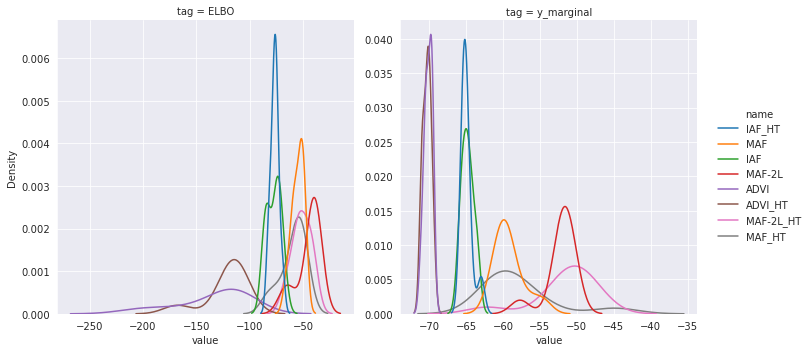
\includegraphics[width=1.0\textwidth]{../Figures/eight_schools.png}
    \begin{subfigure}[t]{0.49\textwidth}
        \centering
        \begin{tabular}{rcc}
            \toprule
                      & ELBO                & $\log p(y)$       \\
            \midrule
            ADVI      & $2873.90 \pm 6.95$    & $2969.73 \pm 1.73$ \\
            TAF       & $2839.64 \pm 9.10$    & $2973.85 \pm 0.87$ \\
            ATAF      & $2842.75 \pm 8.83$    & $2976.75 \pm 0.66$ \\
            NUTS      & n/a                  & $3724.59 \pm 0.036$ \\
            \bottomrule
        \end{tabular}
        \caption{diamonds}
        \label{tab:diamonds}
    \end{subfigure}
    \begin{subfigure}[t]{0.49\textwidth}
        \centering
        \begin{tabular}{rcc}
            \toprule
                      & ELBO                & $\log p(y)$       \\
            \midrule
            ADVI      & $-72.13 \pm 6.89$    & $-53.25 \pm 3.44$ \\
            TAF       & $-64.64 \pm 4.88$    & $-52.51 \pm 4.41$ \\
            ATAF      & $-58.63 \pm 4.75$    & $-51.01 \pm 3.71$ \\
            NUTS      & n/a                  & $-47.78 \pm 0.093$ \\
            \bottomrule
        \end{tabular}
        \caption{Eight schools}
        \label{tab:eight_schools}
    \end{subfigure}

        \caption{Monte-Carlo ELBO and importance weighted Monte-Carlo marginal likelihood
        $p(y) = \EE_{x \sim q_\theta} \frac{p(x,y)}{q_\theta(x)}$ (higher is better, $\pm$ indicates standard errors) 
        estimates from VI on real-world datasets.
        For comparison, we include results computed using ``golden samples'' from \texttt{posteriordb} \citep{ghposteriordb} (NUTS).
        These golden samples are obtained using No-U-Turn-Sampling \citep{hoffman2014no,carpenter2017stan},
        a state-of-the-art MCMC method which does not optimize ELBO, is more computationally expensive than
        VI, and only produces samples rather than parametric probability density functions.
    }
  \label{fig:eight_schools}
  \vspace{-4mm}
\end{table}


\subsection{Non-conjugate BLR on diamonds}
\label{ssec:diamonds}

Without conjugacy, the BLR posterior is intractable and there is no reason \emph{a priori} to expect tail-anisotropy.
Regardless, this presents a realistic and practical scenario for evaluating ATAF's ability to improve VI.
For this experiment, we consider BLR on the \texttt{diamonds} dataset \citep{wickham2011ggplot2} included in
\texttt{posteriordb} \citep{ghposteriordb}.
This dataset contains a covariate matrix $X \in \RR^{5000 \times 24}$ consisting of $5000$
diamonds each with $24$ features as well as an outcome variable $y \in \RR^{5000}$ representing each diamond's price.
The probabilistic model for this inference task is specified in Stan code provided by \citep{ghposteriordb} and is reproduced
for convenience
\begin{gather*}
    \beta \sim \cN(0, \mI_{24}),\quad
    \alpha \sim \text{StudentT}(\nu=3, \text{loc}=8, \text{scale}=10),\quad\\
    \sigma \sim \text{HalfStudentT}(\nu=3, \text{loc}=0, \text{scale}=10),\quad
    y \sim \cN(\alpha + X \beta, \sigma).
\end{gather*}

For each VI method, we performed 100 trials each consisting of 5000 descent steps
on the Monte-Carlo ELBO estimated using 1000 samples and report the results in
\Cref{tab:diamonds}. We report both the final Monte-Carlo ELBO
as well as a Monte-Carlo importance-weighted approximation to
the log marginal likelihood $\log p(y) = \log \EE_{x \sim q_\theta} \frac{p(x,y)}{q_\theta(y)}$
both estimated using 1000 samples.

% \subsection{Bayesian Robust Linear Regression}

% $n = 100$, $d = 10$.

% $X_{ij} \simiid N(0,1)$ for $i \in [n]$, $j \in [d]$.

% $y_i \simiid \text{StudentT}(\text{loc}=X \beta, df=5)$

% Improper ``flat'' prior on $\beta$ to ensure heavy-tailed posterior.

% \begin{figure}[H]
%   \centering
%   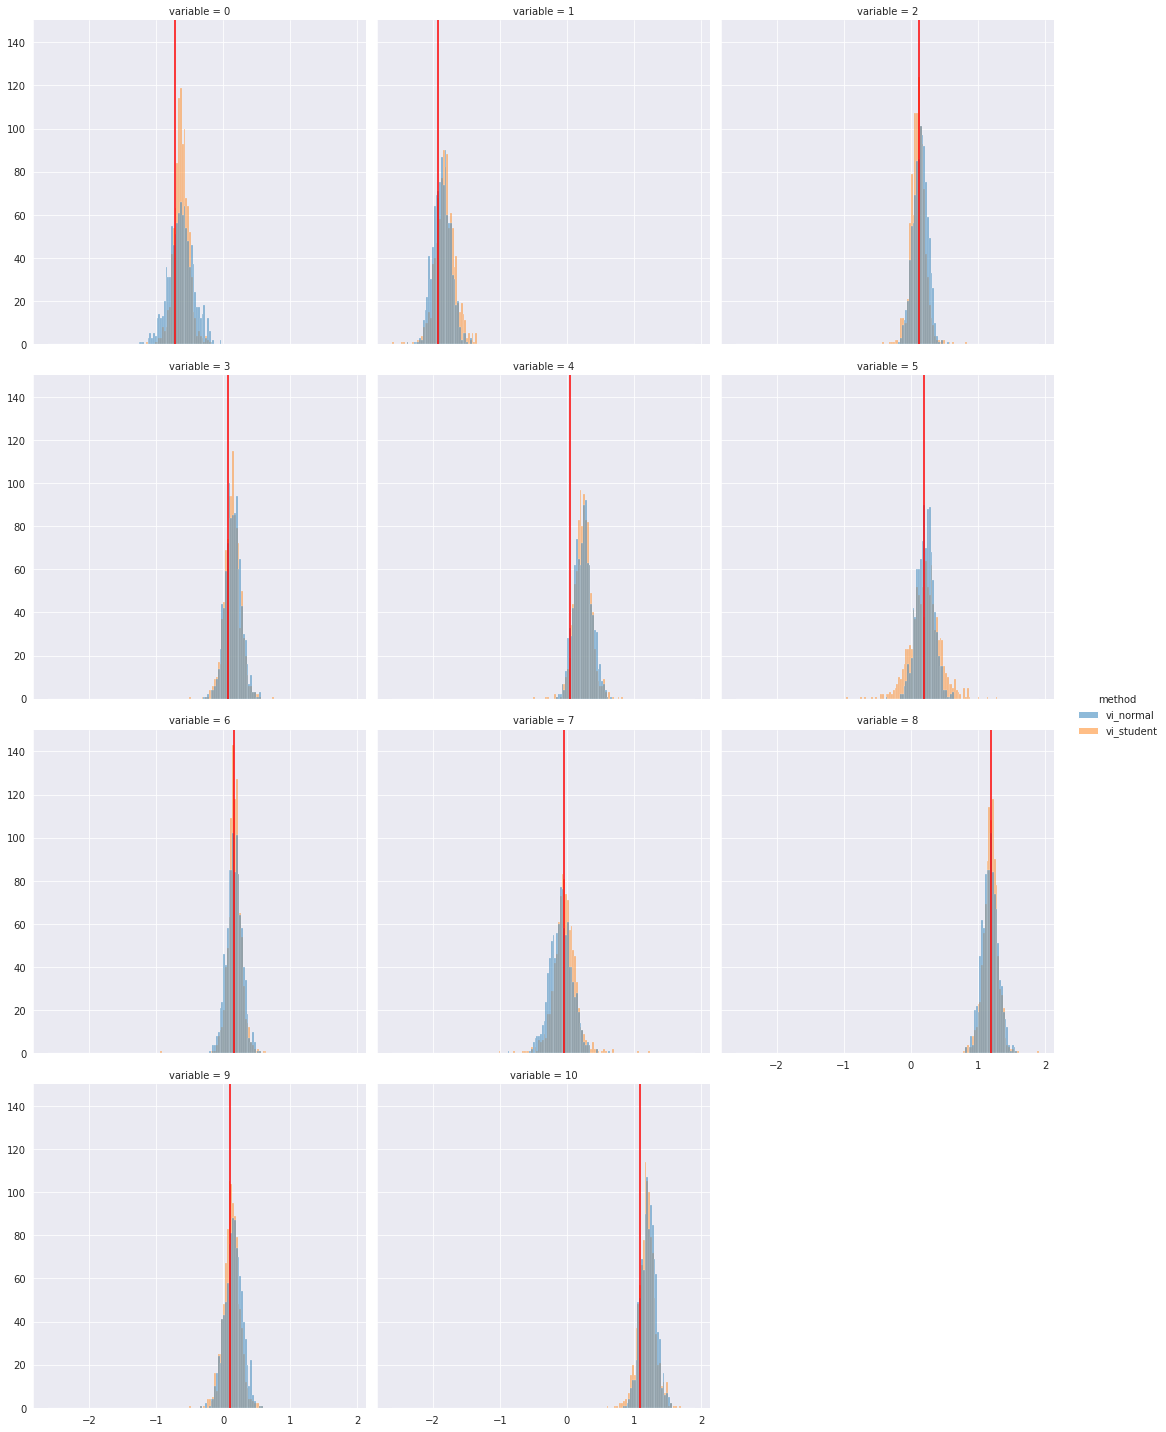
\includegraphics[width=0.9\textwidth]{../Figures/blr.png}
%   \caption{VI of Bayesian robust linear regression}
%   \label{fig:blr}
% \end{figure}

\subsection{Eight schools}
\label{ssec:eight_schools}

The eight-schools model \citep{rubin1981estimation,gelman2013bayesian} is a classical
Bayesian hierarchical model used originally to consider the relationship between standardized
test scores and coaching programs in place at eight schools.
A variation utilizing half Cauchy non-informative priors \citep{gelman2006prior} provides
a real-world inference problem involving fat-tailed distributions, and is formally specified
by the probabilistic model
\begin{align*}
    \mu \sim \cN(0, 5),\quad
    \tau \sim \text{HalfCauchy}(\text{loc}=0, \text{scale}=5),\quad
    \theta \sim \cN(\mu, \tau),\quad
    y \sim \cN(\theta, \sigma).
\end{align*}
Given test scores and standard errors $\{(y_i, \sigma_i)\}_{i=1}^8$, we are interested in the
posterior distribution over treatment effects $\theta_1,\ldots,\theta_d$. The experimental
parameters are identical to \Cref{ssec:diamonds} and results are reported in \Cref{tab:eight_schools}.

% \feynman{TODO}

% \subsection{Bayesian regression analysis on diamonds}
% \feynman{Remove? These are taking too long and don't look good}

% \begin{table}[htbp]
%   \caption{Final ELBO and (MC estimate of) log marginal $\log P(y)$ after 10000 steps on \texttt{diamonds}}
%   \label{fig:blr_diamonds}
%   \centering
%   \begin{tabular}{rcc}
%     \toprule
%               & ELBO   & $\log P(y)$ \\
%     \midrule
%     ADVI      & -374.4 & -6912.0           \\
%     ADVI-HT   & -246.3 & -6876.6     \\
%     MAF       & -211.1 & -6894.8     \\
%     MAF-HT    & -208.5 & -7442.0     \\
%     MAF-2L    & -197.9 & -6532.4     \\
%     MAF-2L-HT & -191.9 & -6839.9     \\
%     MAF-3L    & -194.1 & -7027.3     \\
%     MAF-3L-HT & -209.8 & -7128.1     \\
%     \bottomrule
%   \end{tabular}
% \end{table}


% \feynman{
%   % \subsection{Importance weights}

%   When the importance sampling density is more peaked than the target density.

%   \cite{wang2018variational} example 3.1: Let $p = N(0, \sigma_p^2)$, $q = N(0, \sigma_q^2)$,
%   and for $x \sim q$ let $w(x) = \frac{p(x)}{q(x)}$. If $\sigma_p > \sigma_q$,
%   then $w$ has tail index $\frac{\sigma_p^2}{\sigma_p^2 - \sigma_q^2}$.
%   Otherwise, $w$ is not fat-tailed.
% }

%\section{Related Work}



\section{Conclusion}
\label{sec:conclusion}

We further developed theory on the capability of flow-based methods to represent fat-tailed
target distributions, proposed a direction-dependent tail parameter for the multivariate setting
in order to formalize the idea of tail-(an)isotropy, proved many existing flow-based methods are limited to only represent tail-isotropic distributions, and proposed a new flow-based method called
ATAF which is capable of modeling tail-anisotropic targets.
As we have seen, anisotropic FTVI is already applicable in fairly elementary examples such as Bayesian linear regression
and ATAFs provide one of the first methods for using the representational capacity of flow-based methods
while simultaneously producing tail-anisotropic distributions. We expect the scientific impact of ATAFs to be
fairly easily realized, as it can be applied wherever a parametric density estimator is used.
While we do not expect ATAF to directly have any negative societal impacts,
its broad applicability as a parametric density estimator which accommodates fat-tails means that it may be
used to improve applications which do cause negative societal impact.

% VI is important, FTVI is very important, ADVI did a good job with FTVI, we do a great job with FTVI, and you the reader should follow up on us and do FTVI.

% \begin{ack}
%   Feynman Liang is supported by funding from NPSC and Facebook.
%   Michael Mahoney acknowledges funding from ARO, DARPA, NSF, and ONR.
% \end{ack}
\begin{ack}
  Redacted
\end{ack}


\bibliography{refs_ftvi}

%%%%%%%%%%%%%%%%%%%%%%%%%%%%%%%%%%%%%%%%%%%%%%%%%%%%%%%%%%%%
\section*{Checklist}

%%% BEGIN INSTRUCTIONS %%%
% The checklist follows the references.  Please
% read the checklist guidelines carefully for information on how to answer these
% questions.  For each question, change the default \answerTODO{} to \answerYes{},
% \answerNo{}, or \answerNA{}.  You are strongly encouraged to include a {\bf
%     justification to your answer}, either by referencing the appropriate section of
% your paper or providing a brief inline description.  For example:
% \begin{itemize}
%   \item Did you include the license to the code and datasets? \answerYes{See Section~\ref{gen_inst}.}
%   \item Did you include the license to the code and datasets? \answerNo{The code and the data are proprietary.}
%   \item Did you include the license to the code and datasets? \answerNA{}
% \end{itemize}
% Please do not modify the questions and only use the provided macros for your
% answers.  Note that the Checklist section does not count towards the page
% limit.  In your paper, please delete this instructions block and only keep the
% Checklist section heading above along with the questions/answers below.
%%% END INSTRUCTIONS %%%

\begin{enumerate}

  \item For all authors...
        \begin{enumerate}
          \item Do the main claims made in the abstract and introduction accurately reflect the paper's contributions and scope?
                \answerYes{}
          \item Did you describe the limitations of your work?
                \answerYes{See \Cref{ssec:limitations}}
          \item Did you discuss any potential negative societal impacts of your work?
                \answerYes{See \Cref{sec:conclusion}}
          \item Have you read the ethics review guidelines and ensured that your paper conforms to them?
                \answerYes{}
        \end{enumerate}

  \item If you are including theoretical results...
        \begin{enumerate}
          \item Did you state the full set of assumptions of all theoretical results?
                \answerYes{}
          \item Did you include complete proofs of all theoretical results?
                \answerYes{Deferred to \Cref{sec:proofs}}
        \end{enumerate}

  \item If you ran experiments...
        \begin{enumerate}
          \item Did you include the code, data, and instructions needed to reproduce the main experimental results (either in the supplemental material or as a URL)?
                \answerYes{See \Cref{sec:experiments}}
          \item Did you specify all the training details (e.g., data splits, hyperparameters, how they were chosen)?
                \answerYes{See \Cref{sec:experiments}, \Cref{sec:additional-exp-details}, and open-sourced code}
          \item Did you report error bars (e.g., with respect to the random seed after running experiments multiple times)?
                \answerYes{Tables/figures report standard errors}
          \item Did you include the total amount of compute and the type of resources used (e.g., type of GPUs, internal cluster, or cloud provider)?
                \answerYes{See \Cref{sec:additional-exp-details}}
        \end{enumerate}

  \item If you are using existing assets (e.g., code, data, models) or curating/releasing new assets...
        \begin{enumerate}
          \item If your work uses existing assets, did you cite the creators?
                \answerYes{}
          \item Did you mention the license of the assets?
                \answerYes{See \texttt{LICENSE} and \texttt{README.md} file on Github repository.}
          \item Did you include any new assets either in the supplemental material or as a URL?
                \answerYes{Experiments use newly developed code within \texttt{beanmachine} which is released in \Cref{sec:experiments}.}
          \item Did you discuss whether and how consent was obtained from people whose data you're using/curating?
                \answerNo{Datasets used are either synthetic or released as part of MIT/BSD-3 licensed code.}
          \item Did you discuss whether the data you are using/curating contains personally identifiable information or offensive content?
                \answerNo{We did not screen datasets for PII / offensive content. All experiments perform probabilistic modeling on top of
                existing data, so we do not expect any PII / offensive content to appear in the body of the paper. Please notify us if something
                could potentially make a reader uncomfortable and we will be happy to fix it!
                }
        \end{enumerate}

  \item If you used crowdsourcing or conducted research with human subjects...
        \begin{enumerate}
          \item Did you include the full text of instructions given to participants and screenshots, if applicable?
                \answerNA{}
          \item Did you describe any potential participant risks, with links to Institutional Review Board (IRB) approvals, if applicable?
                \answerNA{}
          \item Did you include the estimated hourly wage paid to participants and the total amount spent on participant compensation?
                \answerNA{}
        \end{enumerate}

\end{enumerate}

%%%%%%%%%%%%%%%%%%%%%%%%%%%%%%%%%%%%%%%%%%%%%%%%%%%%%%%%%%%%
\newpage
\appendix

\section{Proofs}
\label{sec:proofs}

\begin{proof}[Proof of \Cref{thm:distn_class_closed}]
  \label{proof:distn_class_closed}
  Let $X$ be a random variable from either $\cE_\alpha^p$
  or $\cL_\alpha^p$.
  Its concentration function
  \cite[Equation 1.6]{ledoux2001concentration}
  is given by
  \[
    \alpha_X(r)
    \coloneqq \sup \{ \mu\{x : d(x,A) \geq r\}; A \subset \text{supp}~X, \mu(A) \geq 1/2\}
    = \PP(\lvert X - m_X \rvert \geq r)
  \]
  Under Assumption 1, $f_\theta$ is Lipschitz (say with Lipschitz
  constant $L$) so by \cite[Proposition 1.3]{ledoux2001concentration},
  \[
    \PP(\lvert f_\theta(X) - m_{f_\theta(X)}\rvert \geq r)
    \leq 2 \alpha_X(r/L)
    = \cO(\alpha_X(r/L)),
  \]
  where $m_{f_\theta(X)}$ is a median of $f_\theta(X)$.
  Furthermore, by the triangle inequality
  \begin{align}
    \PP(\lvert f_\theta(X) \rvert \geq r)
    &= \PP(\lvert f_\theta(X) - m_{f_\theta(X)} + m_{f_\theta(X)} \rvert \geq r) \nonumber\\
    &\leq \PP(\lvert f_\theta(X) - m_{f_\theta(X)}\rvert \geq r - \lvert m_{f_\theta(X)}\rvert ) \nonumber\\
    &= \cO(\PP(\lvert f_\theta(X) - m_{f_\theta(X)}\rvert \geq r)) \nonumber\\
    &= \cO(\alpha_X(r/L)) \label{eq:pushforward-conc-fn}
  \end{align}
  where the asymptotic equivalence holds because $\lvert m_{f_\theta(X)} \rvert$ is independent of $r$.
  When $X \in \cE_\alpha^p$, \Cref{eq:pushforward-conc-fn} implies
  \[
    \PP(\lvert f_\theta(X) \rvert \geq r)
    = \cO(e^{-\frac{\alpha}{L} r^p}) \implies f_\theta(X) \in \overline{\cE}_{\alpha/L}^p,
  \]
  from whence we find that the Lipschitz transform of exponential-type
  tails continues to possess exponential-type tails with the same
  class index $p$, although the tail parameter may have changed. Hence,
  $\overline{\cE^p}$ is closed under Lipschitz maps for each $p \in \RR_{>0}$.
  On the other hand, when $X \in \cL_\alpha^p$, \Cref{eq:pushforward-conc-fn} also implies that
  \begin{align*}
    \PP(\lvert f_\theta(X) \rvert \geq r)
    &= \cO(e^{-\alpha (\log (r/L))^p}) \\
    &= \cO(e^{-\alpha (\log r)^p} e^{-\alpha (-\log L)^p}) \\
    &= \cO(e^{-\alpha (\log r)^p}),
  \end{align*}
  and therefore, $f_\theta(X) \in \overline{\cL_\alpha^p}$.
  Unlike exponential-type tails, Lipschitz transforms of
  logarithmic-type tails not only remain logarithmic, but
  their tails decay no slower than a logarithmic-type tail
  of the same class index with the \emph{same} tail parameter $\alpha$.
  This upper bound suffices to show closure under Lipschitz maps for the
  ascending family $\overline{\cL_\alpha^p}$.
\end{proof}

\begin{proof}[Proof of \Cref{corr:heavy_to_light}]
    Let $f_\theta$ be as before with the additional assumptions.
    Since $f_\theta$ is a smooth continuous bijection, it is a diffeomorphism.
    Furthermore, by assumption $f_\theta$ has invertible Jacobian on the closure of its
    domain hence $\sup_{x \in \text{dom}~f_\theta} \lvert (f_\theta)'(x) \rvert \geq M > 0$.
    By the inverse function theorem, $(f_\theta)^{-1}$ exists and is
    a diffeomorphism with
    \[
    \frac{d}{dx}(f_\theta)^{-1}(x) = \frac{1}{(f_\theta)'((f_\theta)^{-1}(x))} \leq \frac{1}{M}
    \]
    Therefore, $(f_\theta)^{-1}$ is $M^{-1}$-Lipschitz and we may apply
    \Cref{thm:distn_class_closed} to conclude the desired result.
    %\footnote{\url{https://math.stackexchange.com/questions/394908/diffeomorphism-from-inverse-function-theorem}}
\end{proof}

\begin{proof}[Proof of \Cref{corr:closure_polynomials}]
  Let $X \in \cE^p_\alpha$.
  By considering sufficiently large $X$ such that leading powers dominate, it suffices to consider monomials $Y = X^k$.
  Notice $\PP(Y \geq x) = \PP(X \geq x^{1/k}) = \Theta(e^{-\alpha x^{p/k}})$, and so
  so $Y \in \cE^{p/k}_\alpha$. The result follows by disjointness of $\mathcal{E}$ and $\mathcal{L}$. 
\end{proof}

\begin{lemma}
    \label[lemma]{lem:sum-rule}
    Suppose $X \in \cL^1_\alpha$ and $Y \in \cL^1_\beta$.
    Then $X + Y \in \cL^1_{\min(\alpha,\beta)}$.
\end{lemma}

\begin{proof}
First, let $\gamma=\min\{a,b\}$. It will suffice to show that (I) $\mathbb{P}(|X+Y|\geq r)=\mathcal{O}(r^{-\gamma})$, and (II) $\mathbb{P}(|X+Y|\geq r)\geq\Theta(r^{-\gamma})$. Since $(X,Y)\mapsto|X+Y|$ is a 1-Lipschitz function on $\mathbb{R}^{2}$ and $\mathbb{P}(|X|\geq r)+\mathbb{P}(|Y|\geq r)=\mathcal{O}(r^{-\gamma})$, (I) follows directly from the hypotheses and \cite[Proposition 1.11]{ledoux2001concentration}. To show (II), note that for any $M>0$, conditioning on the event $|Y|\leq M$,\[
\mathbb{P}\left(\left|X\right|+|Y|\geq r\,\vert\,|Y|\leq M\right)\geq\mathbb{P}\left(\left|X\right|\geq r-M\right).
\]
Therefore, by taking $M$ to be sufficiently large so that $\mathbb{P}(|Y|\leq M)\geq\frac{1}{2}$,
\begin{align*}
\mathbb{P}\left(|X+Y|\geq r\right)&\geq\mathbb{P}\left(|X|+|Y|\geq r\right)\\
&\geq\mathbb{P}\left(\left|X\right|+|Y|\geq r\,\vert\,|Y|\leq M\right)\mathbb{P}\left(\left|Y\right|\leq M\right)\\
&\geq\frac{1}{2}\mathbb{P}\left(\left|X\right|\geq r-M\right)=\Theta(r^{-\alpha}).
\end{align*}
The same process with $X$ and $Y$ reversed implies $\mathbb{P}(|X+Y|\geq r)\geq\Theta(r^{-\beta})$ as well. Both (II) and the claim follow.
\end{proof}

\begin{proof}[Proof of \Cref{prop:isotropic-pushforward}]
  Suppose $\mu$ is isotropic, so $\braket{X,v}$ has index $\nu$ for all $v \in \cS^{d-1}$.
  Then for any affine autoregressive flow,
  $\braket{v,f(X)}$ is an affine combination of random variables with tail index $\nu$.
  Note tail parameters are invariant under scalar multiplication as a consequence of
  asymptotic notation, so combined with repeated applications of \Cref{lem:sum-rule} we
  have that the linear combination $\braket{v,f(X)}$ has index $\nu$.
\end{proof}


\section{Normal-normal location mixture}
\label{sec:normal-normal-location-mixture}

We consider a Normal-Normal conjugate inference problem where the posterior
is known to be a Normal distribution as well. Here, we aim to show that ATAF
performs no worse than ADVI because $\text{StudentT}(\nu) \to N(0, 1)$ as $\nu \to \infty$.
\Cref{fig:normal_normal} shows the resulting density approximation, which can
be seen to be reasonable for both a Normal base distribution (the ``correct'' one)
and a StudentT base distribution. This suggests that mis-specification (i.e., heavier
tails in the base distribution than the target) may not be too problematic.

\begin{figure}[H]
  \centering
  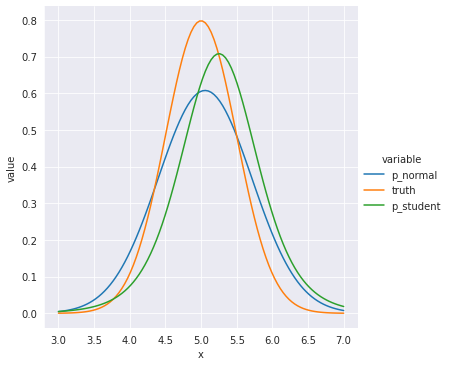
\includegraphics[width=0.6\textwidth]{../Figures/normal_normal_posterior.png}
  \caption{VI against a Normal posterior}
  \label{fig:normal_normal}
\end{figure}


\section{Additional details for experiments}
\label{sec:additional-exp-details}

All experiments were performed on an Intel i8700K with 32GB RAM and a NVIDIA GTX 1080
running PyTorch 1.9.0 / Python 3.8.5 / CUDA 11.2 / Ubuntu Linux 20.04 via Windows Subsystem for Linux.
For all flow-transforms $\Phi_{\text{Flow}}$ we used inverse autoregressive flows \citep{kingma2016improved} with a
dense autoregressive conditioner consisting of varying numbers of hidden layers each with 32 hidden units and
ELU activation functions. Models were trained using the Adam optimizer with $10^{-3}$ learning rate
for 10000 iterations, which we found empirically in all our experiments to result in negligible change in ELBO
at the end of training.

For \cref{tab:diamonds} and \cref{tab:eight_schools}, the flow transform $\Phi_{\text{Flow}}$ used for ADVI, TAF, and ATAF
are comprised of two hidden layers of 32 units each. NUTS uses no such flow transform. Variational parameters
were trained first for ADVI, then used as initialization for TAF. Additionally, the tail parameters $\nu_i$
used in ATAF were initialized to all be equal to the tail parameters learned from training TAF. We empirically observed
this resulted in more stable results (less variation in ELBO / $\log p(y)$ across trials), which may be due to
the absence of outliers when using a Gaussian base distribution resulting in more stable ELBO gradients. This suggests
other techniques for handling outliers such as winsorization may also be helpful, and we leave further investigation
for future work.


For \cref{fig:blr-anisotropic}, the closed-form posterior was computed over a finite element grid to produce
the ``Target'' row. A similar progressive training scheme used for \cref{tab:diamonds} was also used here, with
the TAF flow transform $\Phi_{\text{Flow}}$ was initialized from the result of ADVI and ATAF additionally initialized
all tail parameters $\nu_i$ based on the final shared tail parameter obtained from TAF training. Tails are computed
along the $\beta = 1$ or $\sigma = 1$ axes because the posterior is identically zero for $\sigma = 0$ hence it reveals
no information about the tails.

\end{document}
